\documentclass[a4paper,12pt]{report}

\usepackage[brazilian,english]{babel}
\usepackage{indentfirst}
\usepackage{a4wide}
\usepackage[section]{placeins}
\usepackage[utf8]{inputenc}
% \usepackage[Conny]{fncychap}
\usepackage[T1]{fontenc}
\usepackage{txfonts}
\usepackage{type1cm}
\usepackage{courier}
\usepackage[scaled]{helvet}
\usepackage{epigraph}
\renewcommand*\familydefault{\sfdefault}

\hyphenation{
  es-ta-be-le-ci-do
  a-de-qua-da-men-te
  pro-ble-mas
  di-men-sio-na-men-to
  mo-de-lo
}

% Controlar linhas orfas e viuvas
\clubpenalty=10000
\widowpenalty=10000
\displaywidowpenalty=10000

% Formatar notas de rodape
\usepackage[hang]{footmisc}
\setlength{\footnotemargin}{1em}

\usepackage{url}
%% Define a new 'leo' style for the package that will use a smaller font.
\makeatletter
\def\url@leostyle{%
  \@ifundefined{selectfont}{\def\UrlFont{\sf}}{\def\UrlFont{\small\ttfamily}}}
\makeatother
%% Now actually use the newly defined style.
\urlstyle{leo}

\usepackage[left=3cm,top=3cm,right=2cm,bottom=2cm,includehead,ignoremp]{geometry}

\usepackage[small]{titlesec}
% \titlespacing{\chapter}{0pt}{-50pt}{*20}[0pt]
\titlespacing{\chapter}{0pt}{*-10}{*5}

% Running Headers and footers
\usepackage{fancyhdr}
% \pagestyle{fancy}
\pagestyle{headings}
% Redefine plain page style
\fancypagestyle{plain}{
  \fancyhf{}
  \renewcommand{\headrulewidth}{0pt}
  \fancyhead[LE,RO]{\thepage}
}

\linespread{1.3}
%\pdfpagewidth=\paperwidth
%\pdfpageheight=\paperheight

% Para habilitar cálculos em dimensões
\usepackage{calc}

% Multipart figures
%\usepackage{subfigure}

% More symbols
%\usepackage{amsmath}
%\usepackage{amssymb}
%\usepackage{latexsym}

% Surround parts of graphics with box
\usepackage{boxedminipage}

% Package for including code in the document
\usepackage{listings}

% If you want to generate a toc for each chapter (use with book)
%\usepackage{minitoc}

% This is now the recommended way for checking for PDFLaTeX:
\usepackage{ifpdf}

\ifpdf
\usepackage[pdftex]{graphicx}
\else
\usepackage{graphicx}
\fi

\title{Dionisio}
\author{Allan Douglas R. de Oliveira \\ allandouglas@gmail.com \and
Leonardo Nicacio Bessa \\ leobessa@gmail.com \and
Thiago Rodrigues Andrade \\ suffragiumgmail.com}
\date{2009-04-22}

\usepackage[absolute]{textpos}
\begin{document}

\ifpdf
\DeclareGraphicsExtensions{.png, .pdf, .jpg, .tif}
\else
\DeclareGraphicsExtensions{.eps, .jpg}
\fi

%\maketitle
\pagestyle{empty}
\begin{center}
  {\large ALLAN DOUGLAS R. DE OLIVEIRA \\
    LEONARDO NICACIO BESSA \\
    THIAGO RODRIGUES ANDRADE}
\end{center}

\begin{textblock*}{21cm}[0,0](0cm,12cm)
  \begin{center}
    {\LARGE Dionisio:\\ Um sistema de recomendação baseado em confiança }
  \end{center}
\end{textblock*}


\begin{textblock*}{21cm}[0,0](0cm,29.7cm-4cm)
  \begin{center}
    {\large São Paulo \\ 2009 }
  \end{center}
\end{textblock*}

%\newpage
\begin{center}
  {\large ALLAN DOUGLAS R. DE OLIVEIRA \\
    LEONARDO NICACIO BESSA \\
    THIAGO RODRIGUES ANDRADE}
\end{center}

\begin{textblock*}{21cm}[0,0](0cm,12cm)
  \begin{center}
    {\LARGE Dionisio:\\ Um sistema de recomendação baseado em confiança }
  \end{center}
\end{textblock*}


\begin{textblock*}{21cm}[0,0](0cm,29.7cm-4cm)
  \begin{center}
    {\large São Paulo \\ 2009 }
  \end{center}
\end{textblock*}


\begin{textblock*}{21cm/2-2cm}[0,0](21cm/2,15cm)
  \begin{flushleft}
    {\large
  Monografia apresentada à Escola Politécnica da Universidade de São Paulo para obtenção do título de Bacharel em Engenharia.\newline
  \newline
  Área de Concentração:\newline
  Engenharia de Computação\newline
}
  \end{flushleft}
\end{textblock*}



\begin{center}
  {\large ALLAN DOUGLAS R. DE OLIVEIRA \\
    LEONARDO NICACIO BESSA \\
    THIAGO RODRIGUES ANDRADE}
\end{center}

\begin{textblock*}{21cm}[0,0](0cm,12cm)
  \begin{center}
    {\LARGE Dionisio:\\ Um sistema de recomendação baseado em confiança }
  \end{center}
\end{textblock*}


\begin{textblock*}{21cm}[0,0](0cm,29.7cm-4cm)
  \begin{center}
    {\large São Paulo \\ 2009 }
  \end{center}
\end{textblock*}


\begin{textblock*}{21cm/2-2cm}[0,0](21cm/2,15cm)
  \begin{flushleft}
    {\large
  Monografia apresentada à Escola Politécnica da Universidade de São Paulo para obtenção do título de Bacharel em Engenharia.\newline
  \newline
  Área de Concentração:\newline
  Engenharia de Computação\newline
}

    {\large
      Orientador: Prof. Dr. Jaime Simão Sichman \\
        Co-orientadora: Prof. Dra. Lucia Filgueiras
    }
  \end{flushleft}
\end{textblock*}


%\include{capitulos/01-introducao}

%\begin{textblock*}{21cm/3}[0,0](21cm/3*2-2cm,29.7cm-6cm)
  \begin{flushright}
    {\emph{
           Aos nossos pais e companheiras, pelo apoio e incentivo em nossa formação pessoal. Aos mestres, pelo conhecimento transmitido e pela paciência que tiveram conosco.
          }
    }
  \end{flushright}
\end{textblock*}

\null\newpage


% agradecimentos (opcional)
%\begin{textblock*}{21cm/3}[0,0](21cm/3*2-2cm,29.7cm-6cm)
  \begin{flushright}
\epigraph{\emph{``Innovation distinguishes between a leader and a follower.''}}{Steven Paul Jobs\\Co-fundador da Apple Inc.}
\end{flushright}
\end{textblock*}

\null\newpage


\pagenumbering{roman}

% Resumo e Abstract
\selectlanguage{brazilian}
%  \begin{abstract}
%    O comércio eletrônico brasileiro tem evoluído em termos de serviços prestados ao consumidor. Este trabalho apresenta a especificação e implementação de um sistema online de recomendação para facilitar o encontro do usuário com os produtos e serviços mais relevantes a ele. Para isso, são descritos em detalhes os requisitos funcionais e não funcionais do sistema, os algoritmos de recomendação utilizados e as escolhas na implementação do projeto. 
O sistema projetado é composto por três algoritmos de recomendação, sendo dois deles já difundidos, enquanto o terceiro é um novo, e que foi proposto para levar em consideração as relações de confiança do usuário com seus pares. 
A execução deste trabalho incluiu a realização de um experimento com pessoas interagindo com o sistema de recomendação através de uma rede social. A análise do experimento é apresentada através de gráficos e dados estatísticos que comparam os algoritmos utilizados. 
Os resultados do projeto podem ser aplicados no futuro no desenvolvimento de lojas virtuais online e/ou aplicativos de redes sociais.
%  \end{abstract}
%\begin{otherlanguage}{english}
%  \begin{abstract}
%    The Brazilian e-commerce has evolved in terms of services provided to the consumer. This paper presents the specification and implementation of an online recommendation system that eases the matching of a user with the most relevant products and services. Furthermore the functional and non-functional system requirements, the selected recommendation algorithms and the choices made in the implementation are described in detail.
The designed system consists of three recommendation algorithms, two of them are already widely spreaded, while the third one is new and was proposed to consider the trust among users and their peers.
This work also includes an experiment with people interacting with the recommendation system through a social network. The analysis of the experiment is presented through graphs and statistics that compare the algorithms.
The results of the project can be applied in future development of virtual online stores and/or social networking applications.
%  \end{abstract}
%\end{otherlanguage}

%\listoffigures \thispagestyle{headings} % Lista de Figuras

% \listoftables \thispagestyle{empty} % Lista de Tabelas

\tableofcontents \thispagestyle{headings} % Sumario

% lista de abreviaturas e siglas (opcional)
% lista de simbolos (opcional)

\pagestyle{headings}

% Elementos de Texto
\chapter{INTRODUÇÃO} \pagenumbering{arabic} % (fold)

\section{Objetivo} % (fold)
\label{sec:objetivo}
% Apresentar de forma precisa e concisa o objetivo do projeto.

 O principal objetivo deste projeto é criar um sistema de recomendação baseado em recursos disponíveis na Web, que possibilite a sugestão de itens confiáveis e relevantes ao usuário.

% section objetivo (end)

\section{Motivação} % (fold)
\label{sec:motivação}

% O que é importante para: nós, comunidade científica, usuários, mercado.

% Apresentar a motivação e justificativa para a realização do trabalho (por exemplo, sua aplicabilidade prática, comparação com alternativas já existentes, potencial de  aprendizado e evolução, etc).

% http://www.uxmatters.com/mt/archives/2009/03/including-recommendations-in-user-interfaces-to-enhance-motivation.phps

 Sistemas de Recomendação sugerem aos usuários itens que eles possam gostar, baseado no comportamento prévio do usuário. Fazendo suposições pertinentes sobre o tipo de objetos em que os usuários estão interessados, é possível conquistar a sua confiança. A vantagem para os usuários é a facilidade de encontrar a informação, sem ter a árdua tarefa de procurá-la.

 As redes sociais online têm modificado a forma com que as empresas utilizam a comunicação para o comércio. Pessoas estão utilizando a Web para encontrar outras pessoas com interesses similares, fazer compras de forma mais eficiente, aprender sobre produtos e serviços e reclamar sobre produtos malfeitos\cite{marketing_social_web}.

 A Web está rapidamente se tornando a mídia mais importante para o marketing. A tendência é que as pessoas cada vez mais bloqueiem os anúncios indesejados e queiram ter a capacidade de encontrar os produtos relevantes no momento adequado. É nesse contexto que surge a necessidade de uma plataforma que facilite a colaboração e que permita a criação e classificação de conteúdo pelos consumidores, de forma a permitir uma escolha mais inteligente dos melhores produtos e serviços, e ao mesmo tempo criando uma mecanismo de feedback para as empresas interessadas.

 Devido à grande variedade atual de produtos e serviços, as pessoas têm cada vez mais dificuldade nas suas escolhas e na argumentação sobre a possível decisão. Quanto maior for a quantidade de produtos similares de fabricantes diferentes, mais as pessoas se vêem desnorteadas e sem saber se a decisão realizada foi a mais correta.
 
 % TODO: Escrever sobre Web Semântica

% paragraph paragraph_name (end)
% section motivação (end)

%\section{Organização} % (fold)
%\label{sec:organização}

% Não fazer ainda!!!
% Apresentar a organização do documento: o que cada capítulo, anexo e apêndice aborda.


% section organização (end)

% chapter web_social (end)
%\chapter{ASPECTOS CONCEITUAIS}

\section{O Ambiente} % (fold)
\label{sec:o_ambiente}

\subsection{Cenário}


%\chapter{ESPECIFICAÇÃO DO PROJETO}

\section{Funcionalidades principais}

As funcionalidades principais do dispositivo são:

\begin{itemize}

	\item Captura de vídeo digital a partir de stream MPEG2 de entrada.

	\item Visualização do vídeo capturado na tela do computador.

	\item Interface com outros programas para edição, compressão e armazenamento dos vídeos capturados em diferentes formatos (MPEG, DivX, XVid, entre outros).

	\item Suporte a novos módulos de aplicações para TV Digital (flexibilidade).

	\item Interatividade através de canal de retorno via conexão de Internet.
\end{itemize}

\subsection{Software}
\subsection{Hardware}

%\include{capitulos/4-metodologia}
%\chapter{PROJETO E IMPLEMENTAÇÃO}


%\chapter{TESTES} % (fold)
\label{cha:testes} % (fold)

\section{Descrição do Experimento}
\label{cha:descricao_do_experimento}

 Será feito um experimento para teste do Sistema de Recomendação de Produtos Dionisio.

 Dionisio é um Sistema que armazena informações sobre produtos e pessoas. As pessoas podem formar uma rede social de amigos e avaliar os produtos, fazendo recomendações para outras pessoas conhecidas ou desconhecidas. A partir das avaliações das pessoas e das relações sociais, o sistema gera listas de recomendações de produtos com o objetivo de ajudar as pessoas a encontrar produtos que elas ainda não conhecem mas possuem grande probabilidade de gostar.

 O experimento consistirá de um período de uso do sistema por grupos de pessoas. Serão 12 grupos com 5 pessoas cada um. Os grupos serão formados da seguinte forma:

\begin{itemize}
	\item Inicialmente serão convidadas 12 pessoas de diferentes faixas etárias.
	\item Será passado um endereço de internet (URL) para cada uma das pessoas se cadastrar no sistema
	\item Será pedido a cada uma dessas pessoas que convide mais 4 amigos ou conhecidos, usando uma ferramenta do próprio sistema, para completar um grupo de 5 pessoas.
\end{itemize}

 O cadastro no sistema consiste de um série de formulários que visam extrair informações demográficas e pessoais. Serão pedidas as seguintes informações:
 
\begin{itemize}
	\item Nome
	\item Sexo (masculino ou feminino)
	\item Data de nascimento
	\item Escolaridade
	\item Foto
\end{itemize}

 Será pedido também que elas avaliem em uma escala de 1 a 10, quais são os produtos que elas possuem o maior interesse para obter recomendações, como:

\begin{itemize}
	\item Roupas
	\item Músicas
	\item Filmes
	\item Eletrônicos
	\item Livros
\end{itemize}

	Depois do cadastro dessas informações iniciais será pedido que cada pessoe avalie as outras pessoas de seu grupo, fornecendo as seguintes informações sobre a outra pessoa:

\begin{itemize}
	\item O quanto ela conhece a outra pessoa. As opções são:
	\subitem Não conhece
  \subitem Conhece pouco
  \subitem Conhece bastante
  \subitem Melhor amiga
  \item O quanto ela confia na outra pessoa para a recomendação de produtos em geral:
  \subitem Não confia
	\subitem Confia um pouco
  \subitem Confia muito
  \subitem Confia completamente
\end{itemize}

 Após o levantamento dessas informações será pedido que cada usuário avalie uma série de produtos aleatórios. Cada produto será apresentado através de uma foto e uma descrição. Será pedido que o usuário escolha em uma escala de 1 a 5 o quanto ele gosta daquele produto caso ele o conheça. Se o usuário não conhecer o produto ele deverá escolher a opção "não conheço".

 Feita essa avaliação, começará o uso pleno do sistema pelo usuário. Dentro do sistema as pessoas terão as seguintes opções:
\begin{enumerate}
	\item Ver listas de recomendações
	\item Procurar por produtos
	\item Fazer uma recomendação
	\item Ver lista de pessoas
\end{enumerate}

 Ao acionar a primeira opção será mostrado ao usuário uma série de diferentes listagens de produtos recomendados. Para cada produto recomendado, o usuário terá a opção de avaliar:

\begin{itemize}
	\item O quanto ele gostou daquela recomendação, em uma escala de 1 a 5.
	\item Opcionalmente, o quanto ele gosta daquele produto.
\end{itemize}

 Uma destas listagens será composta pelas recomendações feitas por outras pessoas. Neste caso também será mostrado além do produto recomendado, quem fez a recomendação e uma justificativa do recomendado para aquela recomendação.

 Ao acionar a segunda opção, o usuário poderá ver os diferentes produtos cadastrados no sistema, podendo filtrá-los através de diferentes critérios. Haverá também uma listagem ordenada dos produtos mais bem avaliados nas diferentes categorias de produtos.

 Ao acionar a terceira opção, o usuário poderá fazer uma busca de um produto para recomendar a uma ou mais pessoas cadastradas no sistema. A recomendação consistirá de um produto e de uma justificativa do porquê daquele produto estar sendo recomendado.

 Ao acionar a quarta opção o usuário poderá ver a lista das pessoas conhecidas ou desconhecidas. Inicialmente apenas as pessoas de seu grupo estarão na lista de conhecidos. Mas ele poderá escolher uma outra pessoa para entrar em sua lista de conhecidos fazendo um pedido de amizade.

 A lista de pessoas possui um atalho para o perfil de cada usuário. Este perfil é composto do nome, idade, sexo, foto da pessoa e uma lista dos produtos avaliados por essa pessoa.

 O sistema estará disponível por um período de 1 mês, sendo que ao final o mesmo será desativado e sua base de dados será analisada de forma anônima para se medir qual foi a eficácia das recomendações feitas pelo sistema e entre os usuários.

 \section{Protótipo}
 \label{cha:prototipo}

 Um protótipo do sistema foi desenvolvido para que se pudesse ter noção da usabilidade e do funcionamento do sistema de recomendação. Inicialmente as recomendações são realizadas sem levar em conta os dados de confiança e reputação entre usuários. A Figura~\ref{fig:tela_inicial_prototipo} mostra a página inicial do protótipo, contendo a listagem dos primeiros produtos presentes na base de dados e a opção do usuário fazer o \textit{login} no sistema.
 
\begin{figure}
  \centering
  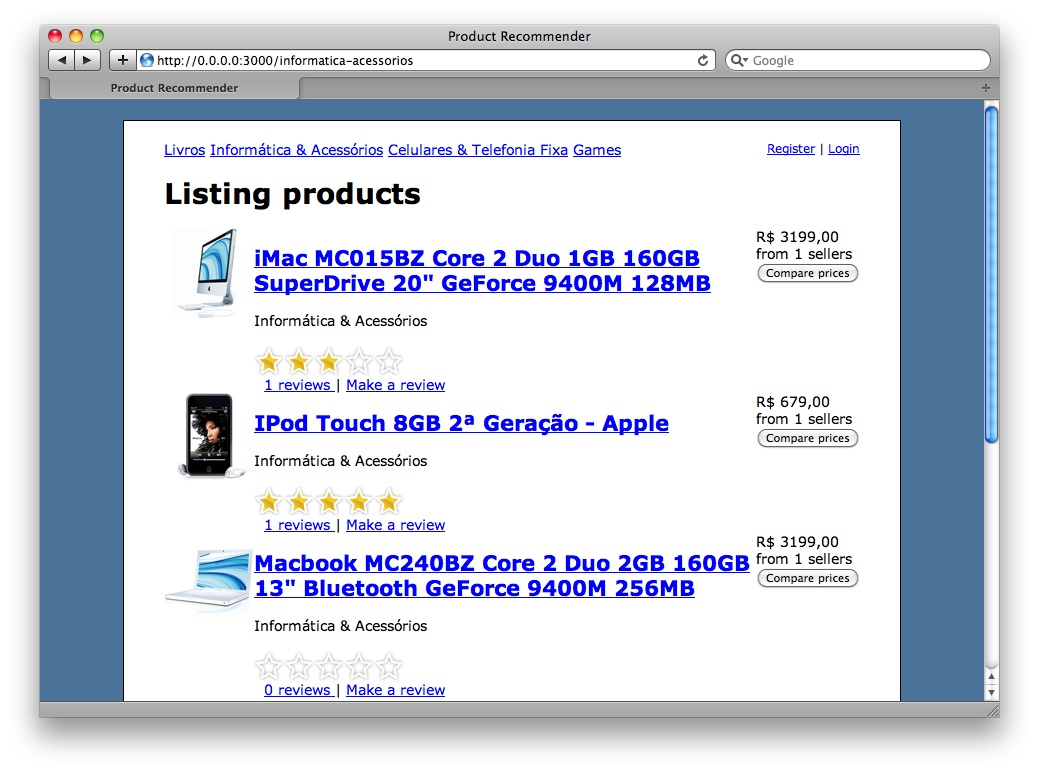
\includegraphics[width=\textwidth]{imagens/Tela_Inicial_Prototipo}
  \caption{\it Tela inicial do protótipo}
  \label{fig:tela_inicial_prototipo}
\end{figure}

 Para se cadastrar, a pessoa necessita apenas informar o seu nome de usuário, e-mail e entrar com uma senha pessoal. A tela de \textit{login} solicita apenas o nome de usuário e senha, conforme ilustrado na Figura~\ref{fig:tela_login_prototipo}. Após a validação dos dados, o sistema retorna para a tela inicial para que o usuário possa detalhar um produto de seu interesse. Há a opção de avaliar o produto sem conferir os seus detalhes. Para avaliar o produto o usuário escolhe de 1 a 5, sendo 1 não gostar do produto e 5 gostar muito, e clicar em uma das cinco estrelas. O número de estrelas coloridas mostra a nota da avaliação. 
 
 Para efetuar o \emph{login} o sistema solicita apenas o nome de usuário e senha. Após a autenticação, o sistema retorna para a tela inicial para que o usuário possa procurar um produto de seu interesse. Ao escolher um produto, o sistema abre os seus detalhes incluindo nome, foto e descrição completa, como mostra a Figura~\ref{fig:detalhe_produto_prototipo}.

\begin{figure}
  \centering
  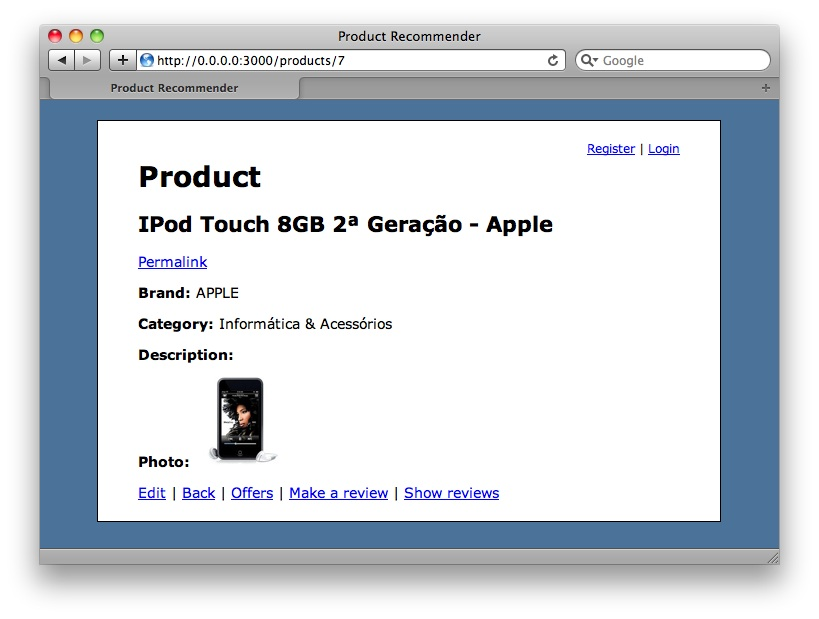
\includegraphics[width=\textwidth]{imagens/Detalhe_Produto_Prototipo}
  \caption{\it Detalhe do produto}
  \label{fig:detalhe_produto_prototipo}
\end{figure}

 Na tela de detalhamento do produto o usuário poderá editar as informações do mesmo ao escolher a opção \textit{edit}. Também é possível visualizar os comentários (\textit{reviews}) feitos pelos usuários sobre o produto detalhado, além de fazer o seu próprio comentário, clicando em \textit{Make a review}.
  
 A encontrar um produto interessante o usuário tem a opção de recomendá-lo para outros da rede social. A opção \emph{Recommend it!} leva o usuário a tela ilustrada na Figura~\ref{fig:recomendacao_produto_prototipo}, onde é possível selecionar os amigos para os quais a recomendação será enviada.

 \begin{figure}
   \centering
   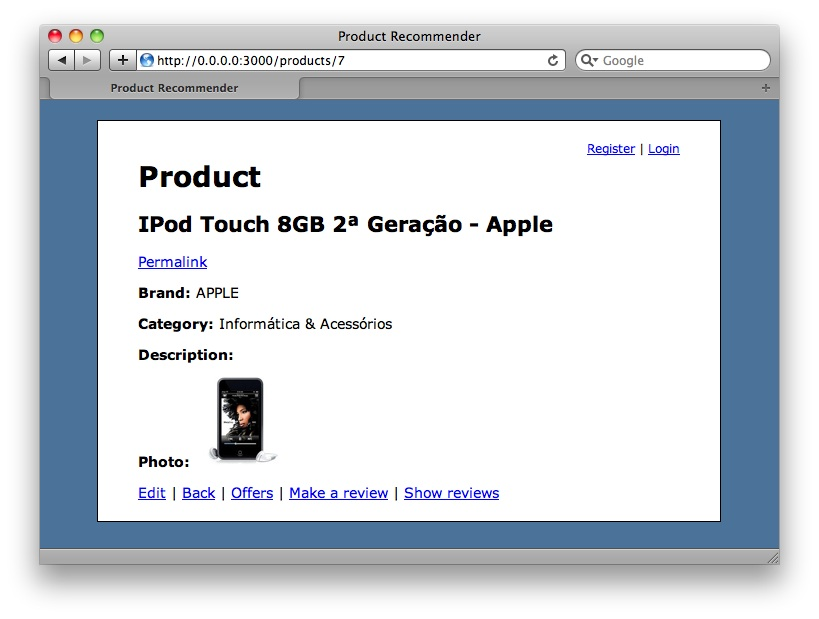
\includegraphics[width=\textwidth]{imagens/Detalhe_Produto_Prototipo}
   \caption{\it Detalhe do produto}
   \label{fig:detalhe_produto_prototipo}
 \end{figure}         
 
 \begin{figure}
   \centering
   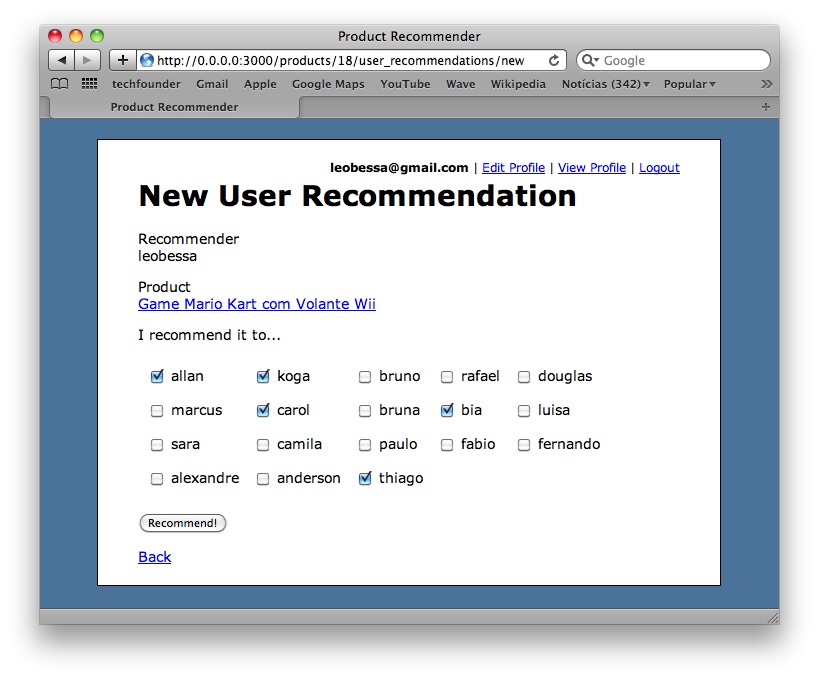
\includegraphics[width=\textwidth]{imagens/TELA_RECOMENDACAO_PROTOTIPO}
   \caption{\it Tela de recomendação de produto}
   \label{fig:recomendacao_produto_prototipo}
 \end{figure}

%\chapter{CONSIDERAÇÕES FINAIS}

\section{Análise dos Resultados} % (fold)
\label{sec:analise_resultados}
% section analise_resultados (end)

\section{Trabalhos Futuros} % (fold)
\label{sec:trabalhos_futuros}

% section trabalhos_futuros (end)


\addcontentsline{toc}{chapter}{Referências Bibliográficas}
\bibliographystyle{abnt-num}   %\bibliographystyle{plain}
% \bibliography{bibname.bib} % bibname=nome do seu arquivo BibTeX
\begin{thebibliography}{99}

 

%  \bibitem{marketing_social_web}
%    WEBER, LARRY.
%    \textbf{Marketing to the social web}: how digital customer communities build your business.
%    Wiley, 2007, 5 p.

\end{thebibliography}


%\addcontentsline{toc}{chapter}{Glossário}
%\chapter*{Glossário} % (fold)
\label{cha:glossario}

\begin{itemize}

  \item \emph{ADSL}: acrônimo de \emph{Asymmetric Digital Subscriber Line}, é uma forma de transmissão de dados de alta velocidade utilizando linhas telefônicas comuns, em freqüências maiores que os seres humanos conseguem escutar.

  \item \emph{BNC}: é um tipo de conector cujo nome vem de seus criadores: ``bayonet Neil-Concelman''. Sua grande característica é o sistema de trava, tipo twist-lock (gira e trava), que possibilita grande segurança na conexão. É bastante utilizado nos equipamentos profissionais de vídeo.

  \item \emph{Broadcast}: é um modo de difusão de sinais em que é transmitido o mesmo conteúdo para todos os receptores. Numa transmissão de TV, por exemplo, todas as pessoas sintonizadas no mesmo canal assistem ao mesmo programa. Em Internet, o termo é usado muitas vezes para designar o envio de uma mensagem par todos os membros de um grupo, em vez da remessa para membros específicos.

  \item \emph{Buffer}: é uma área de armazenamento que compensa diferentes velocidades de fluxos de dados ou temporizações de eventos, ao transferir dados de um dispositivo para outro.

  \item \emph{CD}: acrônimo de Compact Disc, é um padrão de armazenamento óptico para dados digitais.
  Conversor A/D: um Conversor Analógico-Digital é componente de um sistema responsável por converter dados analógicos para digitais através da amostragem de um sinal contínuo e sua posterior discretização gerando valores numéricos digitais.

  \item \emph{Classpath}: é um argumento passado para a Java Virtual Machine indicando onde procurar classes e pacotes para carregamento dinâmico.

  \item \emph{CPqD}: {C}entro de {P}es{q}uisa e {D}esenvolvimento em Telecomunicações.

  \item \emph{DivX}: é um formato de compactação de vídeo criado pela DivxNetworks Inc.

  \item \emph{Driver}: um driver é um componente de software responsável por estabelecer a comunicação entre hardware e software, provendo comandos para enviar e receber dados de um dispositivo instalado.

  \item \emph{DVD}: acrônimo de Digital Versatile Disc, é a geração seguinte ao CD, possibilitando um armazenamento maior de dados.

  \item \emph{ECMAScript}: é uma linguagem de programação baseada em scripts, padronizada pela Ecma International na especificação ECMA-262. A linguagem é bastante usada em tecnologias para Internet, sendo esta base para a criação do JavaScript/JScript e também do ActionScript.

  \item \emph{FIFO}: acrônimo para {F}irst {I}n, {F}irst {O}ut (que em português significa primeiro a entrar, primeiro a sair) refere-se a estruturas de dados do tipo fila onde os elementos vão sendo colocados e retirados (ou processados) por ordem de chegada.

  \item \emph{GEM}: acrônimo de \emph{Globally Executable MHP} \cite{gem}, é uma parte do MHP independente dos padrões de transmissão europeus, criado com a finalidade de padronizar partes de todos os padrões de \emph{middleware} mundiais e possibilitar a criação de aplicações que funcionem em qualquer \emph{middleware} que seja compatível com o GEM.

  \item \emph{GSM}: acrônimo de Global System for Mobile Communications é um dos principais padrões para telefonia móvel existente.

  \item \emph{Heap}: Heap de objetos é o nome dado a parte da memória do computador que contém a estrutura de dados responsável por armazenar todos os objetos durante a execução da máquina virtual Java.

  \item \emph{HTTP}: acrônimo para {H}yperText {T}ransfer {P}rotocol (Protocolo de Transferência de Hipertexto), utilizado para transferência de dados na rede mundial de computadores, a World Wide Web.

  \item \emph{IPC (Inter-Process Communication)}: é o grupo de mecanismos que permite aos processos transferirem informação entre si. Entre estes mecanismos podem ser citados pipes, filas de mensagens e memória compartilhada.

  \item \emph{Java}: é uma linguagem de programação orientada a objeto desenvolvida na década de 90 pelo programador James Gosling, na empresa Sun Microsystems.

  \item \emph{JavaBeans}: são componentes reutilizáveis de software escritos em linguagem Java, e que seguem algumas convenções de modo a permitir que ferramentas possam utilizá-los e manipulá-los.

  \item \emph{JavaTV}: é uma biblioteca Java que contempla a maior parte dos recursos necessários para a operação de sistemas receptores de TV digital, simplificando assim o desenvolvimento de softwares, uma vez que os programadores de aplicativos podem se voltar ao tema principal da aplicação em desenvolvimento.

  \item \emph{JNI (Java Native Interface)}: é um padrão de programação que permite que a máquina virtual da linguagem Java acesse bibliotecas construídas com o código nativo de um sistema.

  \item \emph{Lista ligada}: é uma estrutura de dados linear e dinâmica composta por células que apontam para o próximo elemento da lista.

  \item \emph{Metodologia (Processo) de Desenvolvimento Ágil}: metodologias de desenvolvimento ágil foram pensadas de forma a minimizar riscos no desenvolvimento de software através períodos mais curtos de lançamento, chamados iterações, que tipicamente levam de uma quatro semanas. Métodos ágeis prezam mais a comunicação face-a-face que a documentação, como forma de acelerar o processo de desenvolvimento.

  \item \emph{MHP}: acrônimo de \emph{Multimedia Home Platform} \cite{mhp}, é um padrão aberto de \emph{middleware} para TV Digital, adotado principalmente pelos países europeus. Está incluso em outro padrão maior, o \emph{Digital Video Broadcasting} (DVB) \cite{dvb} que agrupa todas as características da tecnologia de TV Digital européia.

  \item \emph{Middleware} (conforme \cite{ginga}): é a camada de software intermediário que permite o desenvolvimento de aplicações interativas para a TV Digital de forma independente da plataforma de hardware dos fabricantes de terminais de acesso (\emph{set-top boxes}).

  \item \emph{MPEG}: acrônimo para {M}oving {P}icture {E}xperts {G}roup, é o grupo de trabalho da Organização Internacional para Padronização (ISO) para o desenvolvimento de padrões para vídeo e áudio digitais.

  \item \emph{MPEG2}: é um padrão de compressão e codificação de vídeo para difusão e comunicações, bem como para armazenamento em meios diversos, tais quais os ópticos.

  \item \emph{MPEG-TS}: MPEG {T}ransport {S}tream (TS, TP, ou MPEG-TS) é um protocolo de  comunicação para transmissão de áudio, vídeo e dados, especificado pelo padrão  ISO/IEC 13818-1. Permite multiplexar vídeo e áudio digital sincronizando a saída. Possui correção de erro e transporte, e é usado para difusão de aplicações como DVB e ATSC.

  \item \emph{MOV}: formato de vídeo criado pela Apple, é um container para imagem, diversas trilhas, efeitos e textos. Sua base foi aprovada pela ISO como padrão para MPEG4 Part. 14.

  \item \emph{Multiplexação no tempo}: a multiplexação no tempo consiste na transmissão de dois ou mais sinais ou fontes de bits simultaneamente através de um único canal pela divisão do tempo em pequenos compartimentos de tamanhos fixos, onde são transmitidos alternadamente um pouco de cada sinal.

  \item \emph{Overhead}: Em computação overhead é geralmente considerado qualquer processamento ou armazenamento em excesso, seja de tempo de computação, de memória, de largura de banda ou qualquer outro recurso que seja requerido para ser utilizado ou gasto para executar uma determinada tarefa.

  \item \emph{Pipe (UNIX)}: é o redirecionamento da saída padrão de um programa para a entrada padrão de outro.

  \item \emph{{S}et-{t}op {B}ox ({STB})}: é o termo que descreve um equipamento que se conecta a um televisor e a uma fonte externa de sinal, transformando este sinal em conteúdo no formato que possa ser apresentado em uma tela.

  \item \emph{SBTVD} \cite{sbtvd}: acrônimo para {S}istema {B}rasileiro de {TV} {D}igital.

  \item \emph{SMS}: acrônimo para {S}hort {M}essage {S}ervice. Tecnologia amplamente utilizada em telefonia celular para a transmissão de mensagens de texto curtas.

  \item \emph{SOAP}: acrônimo de \emph{Service Oriented Architecture Protocol}, é um protocolo de troca de mensagens em formato XML.

  \item \emph{Thread}: é uma forma de um processo dividir a si mesmo em duas ou mais tarefas que podem ser executadas simultaneamente.

  \item \emph{UML}: acrônimo de Unified Modelling Language, é um padrão gráfico de especificação para modelagem de objetos, e uma ferramenta importante no processo de desenvolvimento de software.

  \item \emph{{USB}}: acrônimo de {U}niversal {S}erial {B}us, é uma especificação para interfaces de comunicação serial de dados. É padronizado pelo {USB} {I}mplementers {F}orum ({USB-IF}), que possui membros como Apple Inc., Hewlett-Packard, NEC, Microsoft e Intel.

  \item \emph{W3C}: acrônimo de World Wide Web Consortium, é o principal órgão de padronização para a Web (Internet).

  \item \emph{Web Services}: é definido pelo W3C como um sistema de software projetado para dar suporte à comunicação interoperável entre duas máquinas utilizando uma rede. Essa comunicação é feita através de mensagens XML utilizando-se servidores web, em um padrão denominado SOAP.

  \item \emph{Wi-Fi}: é uma marca registrada pertencente à Wireless Ethernet Compatibility Alliance (WECA), e é a abreviatura de \emph{wireless fidelity}, sendo uma tecnologia de interconexão entre dispositivos sem fio, usando o protocolo IEEE 802.11.

  \item \emph{WiMax}: acrônimo de \emph{Worldwide Interoperability for Microwave Access}, é o nome comercial para o padrão IEEE 802.16, que especifica uma interface sem fio para redes metropolitanas, agregando conhecimentos e recursos mais recentes ao padrão Wi-Fi visando melhor performance de comunicação.

  \item \emph{WMV}: \emph{Windows Media Video} é o nome para uma série de formatos de vídeo compactados criados pela Microsoft.

  \item \emph{XHTML}: acrônimo para \emph{eXtensible HyperText Markup Language}, é uma linguagem de marcação com as mesmas marcas do HTML, porém com uma sintaxe mais rigorosa pois é baseada no XML, e dessa podem ser validadas com bibliotecas XML.

  \item \emph{XML}: acrônimo para \emph{eXtensible Markup Language}, é uma especificação para uma linguagem de marcação de uso geral, permitindo que possam ser criados novas linguagens.

  \item \emph{XviD}: formato de compactação de vídeo competidor direto do DivX. Enquanto o DivX é um formato proprietário, o XVid é livre e de código aberto, disponível para diferentes plataformas.

  \item \emph{YouTube}: é um site na Internet que permite que seus usuários carreguem, assistam e compartilhem vídeos em formato digital. Foi fundado em fevereiro de 2005 por três pioneiros do PayPal, um famoso site da internet ligado a gerenciamento de doações. Foi comprada em 9 de Outubro de 2006 pelo Google, pela quantia de US\$1,65 bilhões em ações.

\end{itemize}
% chapter glossário (end)



% anexos (opcional)
%\addcontentsline{toc}{chapter}{\appendixname}
%\appendix
%

%


% indice remissivo (opcional)

\end{document}
